\documentclass[14pt]{extarticle}
\usepackage[utf8x]{inputenc}
\usepackage[english,russian]{babel}
\usepackage{indentfirst}
\usepackage{graphicx}
\usepackage{verbatim}
\usepackage{amsmath}
\usepackage{amsfonts}
\usepackage{longtable}
\usepackage[a4paper,margin=1.0in,footskip=0.25in]{geometry}

\makeatletter
\newcommand{\verbatimfont}[1]{\renewcommand{\verbatim@font}{\ttfamily#1}}
\author{Даниил Крачковский}
\title{Отчёт по преддипломной практике}

% Change table of contents title
\addto\captionsrussian{\renewcommand{\contentsname}{Оглавление}}

\begin{document}

\begin{titlepage}

\newpage

\begin{center}
МИНИСТЕРСТВО ОБРАЗОВАНИЯ РЕСПУБЛИКИ БЕЛАРУСЬ \\
БЕЛОРУССКИЙ ГОСУДАРСТВЕННЫЙ УНИВЕРСИТЕТ \\
Факультет прикладной математики и информатики \\
Кафедра вычислительной математики
\end{center}

\vspace{8em}
    
    \begin{center}
    \Large Крачковский Даниил Янович
    \end{center}

    \begin{center}
    \Large Вычислительные алгоритмы положительной матричной факторизации
    \end{center}

    \vspace{2.5em}

    \begin{center}
    	Отчет о преддипломной практике \\
    	студента 4 курса 5 группы
    \end{center}

    \vspace{6em}
    
    \begin{flushright}
    	Научный руководитель \\
		Фалейчик Борис Викторович
    \end{flushright}
    
    \vfill

    \begin{center}
    	Минск 2019
    \end{center}

    \end{titlepage}

\tableofcontents


\newpage


\section{Введение}
На сегдняшний день объемы информации растут в геометрической прогрессии. Ярким примером  скопления обширного количества данных является социальная сеть Instagram переступившая порог в 1 млрд пользователей. Для того чтобы быстрее реагировать на изменения рынка, получить конкурентные преимущества, повысить эффективность сервиса нужно получить, обработать и проанализировать огромное количество данных. Обработка таких больших объемов данных создаёт новые проблемы в отношении представления данных, упразднения неоднозначности и уменьшения размерности.

Во многих ситуациях данные, наблюдаемые из сложных процессов и взаимодействий представляют собой совокупный результат нескольких взаимосвязанных переменных, действующих вместе. Когда эти переменные определены с некоторыми неточностями, фактическая информация, содержащаяся в исходных данных, может перекрываться и быть неоднозначной. В данном случае модель с упрощённой системой может обеспечить точность около уровня точности исходной системы. Одна общая идея в различных подходах к устранению шума, уменьшению размерности модели, восстановлению непротиворечивости и т.д. заключается в замене исходных данных данными меньшей размерности, полученными с помощью аппроксимации некоторым подпространством. Эта идея получила название `low-rank approximation`. Использование `low-rank approximation` выходит на передний план в широком спектре важных задач. Факторный анализ и метод главных компонент являются двумя из многих классических методов, используемых для достижения цели сокращения числа переменных и выявления структур среди переменных.

Часто анализируемые данные неотрицательны, что накладывает следующие ограничения на аппроксимирующие данные: данные более низкого ранга также должны состоять из неотрицательных значений, чтобы избежать противоречий с природой исходных данных. Классические инструменты не могут гарантировать сохранение неотрицательности. Таким образом, естественным выбором становится поиск неотрицательных множителей пониженного ранга для аппроксимации данной неотрицательной матрицы данных. Это является, так называемой, проблемой положительной матричной факторизации.

\newpage


\section{Постановка задачи}

Для матрицы $A \in R^{m \times n}, A \geq 0$ и числа $k \in N, k < min\{n, m\}$ необходимо найти матрицы $W \in R^{m \times k}, H \in R^{k \times n} : W \geq 0, H \geq 0$ чтобы свести к минимуму функционал:
$$
f(W, H) = \dfrac{||A - WH||_F}{|| A ||_F}
$$
Произведение $WH$ называется положительной факторизацией матрицы $A$. В идеальном случае, когда $f(W,H) = 0$ матрица $A$ равна произведению $WH$. На практике это далеко не всегда так, и почти всегда произведение $WH$ является приближенным разложением ранга не более $k$.


\newpage


\section{Исследования задачи}

Правильный выбор значения $k$ является критически важным для получения удовлетворительного результата, но также выбор $k$ очень часто зависит от природы решаемой задачи и поставленного вопроса. В большинстве случаев, $k$ обычно выбирают таким образом, чтобы $k \ll min\{m, n\}$, и в этом случае произведение $WH$ можно рассматривать как сжатую форму данных матрицы $A$. 

Ключевой характеристикой положительной матричной факторизации является возможность использования численных методов для минимизации $f(W,H)​$ для извлечения некоторых базовых признаков в качестве базисных векторов матрицы $W​$, которые затем могут быть использованы для поиска и классификации. Ограничивая матрицы $W​$ и $H​$ только неотрицательными элементами положительная матричная факторизация позволяет представлять исходные данные из не вычитающих комбинаций. Элементы таких комбинаций могут быть частями лиц в изображениях, темами или кластерами в текстовых данных или некоторыми другими характеристиками многомерных данных.

Одной их важных проблем, влияющих на численную минимизацию $f(W, H)$, является существование локальных минимумов из-за невыпуклости $f(W, H)$ как по $W$, так и по $H$. Не менее важной проблемой является отсутствие единственного решения, которое можно легко увидеть рассматривая произведение $WDD^{− 1}H$ для любой неотрицательной обратимой матрицы $D$. 

Несмотря на многие недостатки положительная матричная факторизация весьма привлекательна для приложений интеллектуального анализа данных, поскольку на практике даже локальные минимумы могут обеспечивать желаемые свойства, такие как сжатие данных и извлечение базовых признаков. 


\newpage


\section{Алгоритмы}

Численные алгоритмы положительной матричной факторизации могут быть поделены на 3 основные категории:
\begin{enumerate}
	\item Мультипликативные алгоритмы / Multiplicative update
	\item Алгоритмы градиентного спуска / Gradient descent
	\item Алгоритмы попеременных наименьших квадратов / Alternating least squares
\end{enumerate}

В ходе работы были исследованы 2 категории алгоритмов: мультипликативные алгоритмы и алгоритмы попеременных наименьших квадратов. Далее рассмотрим некоторые примеры из этих категорий подробнее.

Изложенные ниже алгоритмы предполагают изначальное заполнение матриц $W$ и $H$ случайными, неотрицательными числами.


\newpage


\subsection{Multiplicative update rule}

Алгоритм был разработан и улучшен Daniel D. Lee и H. Sebastian Seung в 2001 году.

\begin{align*}
	& H_{i+1} = H_i * W_i^T A / (W_i^T W_i H_i + \epsilon) \\
	& W_{i+1} = W_i * A H_{i+1}^T / (W_i H_{i+1} H_{i+1}^T + \epsilon) & i = 1, 2, ...
\end{align*}

Ниже приведена реализация алгоритма на `python3`:

\verbatimfont{\small}
\begin{verbatim}
eps = 10e-9

while True:
  # H = H * (W' A) / ((W' W H) + 10e-9)
  expr1 = W.T @ A
  expr2 = (W.T @ W) @ H + eps
  H = element_wise_divide(element_wise_multiply(H, expr1), expr2)

  # W = W * (A H') / ((W H H') + 10e-9)
  expr3 = A @ H.T
  expr4 = W @ (H @ H.T) + eps
  W = element_wise_divide(element_wise_multiply(W, expr3), expr4)

  yield relative_error(A, W, H)
\end{verbatim}


\newpage


\subsection{Alternating least squares}

В этом алгоритме за шагом наименьших квадратов следует другой шаг наименьших квадратов поочередно. Алгоритм использует тот факт, что задача минимизации выражения $f(W, H)$ не является выпуклой как в $W$, так и в $H$ одновременно, но является выпуклой в $W$ или $H$ по отдельности. Таким образом, для одной матрицы другая матрица может быть найдена с простым вычисление наименьших квадратов.

\begin{align*}
	& H_{i+1} = solve(W_i^T W_i H_{i+1} = W_i^T A) \\
	& H_{i+1} = nonnegative(H_{i+1}) \\
	& W_{i+1}^T = solve(H_{i+1} H_{i+1}^T W_{i+1}^T = H_{i+1} A^T) \\
	& W_{i+1} = nonnegative(W_{i+1}) & i = 1, 2, ...
\end{align*}

Ниже приведена реализация алгоритма на `python3`:

\verbatimfont{\small}
\begin{verbatim}
while True:
  # W' W H = W' A
  H = solve(W.T @ W, W.T @ A)
  H = nonnegative(H)

  # H H' W' = H A'
  WT = solve(H @ H.T, H @ A.T)
  W = nonnegative(WT.T)

  yield relative_error(A, W, H)
\end{verbatim}


\newpage


\subsection{Алгоритм инициализации матриц $W$ и $H$}

Проблема изложенных алгоритмов положительной матричной факторизации заключается в том, что сходимость к глобальному минимуму не гарантируется. Часто случается, что сходимость медленная и достигается неоптимальное приближение. 

Эффективная процедура для вычисления хорошего начального приближения может быть основана на сингулярном разложении матрицы $A$.

Если $A = U \Sigma V^T $ является сингулярным разложением для матрицы $A$, мы можем взять первый сингулярный вектор $u_1$ в качестве первого столбца в $W$. Затем мы вычисляем матрицу $C = u_2 v_2^T$ и заменяем все отрицательные её элементы на ноль. Т.к. $C$ теперь является неотрицательной матрицей, то мы знаем, что первый сингулярный вектор этой матрицы также неотрицательный. Кроме того, мы можем надеяться, что это достаточно хорошее приближение $u_2$, поэтому мы можем принять его за второй столбец $W$. Продолжим процедуру дальше, пока не заполним всю матрицу $W$.

Ниже приведена реализация алгоритма на `python3`:

\verbatimfont{\small}
\begin{verbatim}
rows, columns = A.shape

U, _, VT = svd_factorization(A, rank_k)

W = U[:,:rank_k]
H = random_matrix(rank_k, columns)

for j in range(1, rank_k):
  C = reshape(U[:,j], (rows, 1)) @ reshape(VT[j,:], (1, columns))
  C = nonnegative(C)
  u, _, _ = svd_factorization(C, 1)

  W[:,j] = u[:,0]
return W, H
\end{verbatim}


\newpage

\section{Эксперимент}

\iffalse
Term-document matrices are used in information retrieval. Con-
sider the following selection of five documents. 1 Key words, which we call terms,
are marked in boldface.

\begin{longtable}{ l p{10cm} }
 Документ 1: & Progressive \textbf{Web} \textbf{Applications} are experiences that combine the best of the \textbf{web} and the best of \textbf{applications}. \\
 Документ 2: & The number of \textbf{transactions} in the Bitcoin \textbf{blockchain} has reached a historical maximum.\\ 
 Документ 3: & The reason why the Progressive \textbf{Web} \textbf{Applications} ecosystem of \textbf{tooling} seems overwhelming is because it’s always explained in the wrong \textbf{order}.\\
 Документ 4: & PayPal made the first \textbf{investment} in a \textbf{startup} working with \textbf{blockchain} \textbf{technology}.\\
 Документ 5: & Belarusian \textbf{startup} released an \textbf{application} that allows you to ``try on'' new \textbf{sneakers} before you buy them.\\  
 Документ 6: & The new level of \textbf{quality} allows Progressive \textbf{Web} \textbf{Applications} to earn a place on the user's \textbf{home} screen. \\
\end{longtable}



\begin{center}
 \begin{tabular}{ l | c c c c c c } 
 Term        & Док 1 & Док 2 & Док 3 & Док 4 & Док 5 & Док 6 \\
 \hline
 home        & 0 & 0 & 0 & 0 & 0 & 1 \\ 
 web         & 2 & 0 & 1 & 0 & 0 & 1 \\
 tool        & 0 & 0 & 1 & 0 & 0 & 0 \\ 
 order       & 0 & 0 & 0 & 0 & 0 & 0 \\ 
 investment  & 0 & 0 & 0 & 1 & 0 & 0 \\ 
 startup     & 0 & 0 & 0 & 1 & 1 & 0 \\ 
 transaction & 0 & 1 & 0 & 0 & 0 & 0 \\
 technology  & 0 & 0 & 0 & 1 & 0 & 0 \\ 
 application & 2 & 0 & 1 & 0 & 1 & 1 \\ 
 sneaker     & 0 & 0 & 0 & 0 & 1 & 0 \\ 
 quality     & 0 & 0 & 0 & 0 & 0 & 1 \\ 
 blockchain  & 0 & 1 & 0 & 1 & 0 & 0 \\
\end{tabular}
\end{center}
\fi

Терм-документная матрица представляет собой матрицу, описывающую частоту терминов, которые встречаются в коллекции документов. Такие матрицы используются при поиске информации. Рассмотрим следующую подборку из пяти документов \cite{elden}. Ключевые слова, которые мы называем терминами,
выделены жирным шрифтом.

\begin{longtable}{ l p{12cm} }
 Документ 1: & The \textbf{Google} \textbf{matrix} $P$ is a model of the \textbf{Internet}. \\
 Документ 2: & $P_{ij}$ is nonzero if there is a \textbf{link} from \textbf{Web} \textbf{page} $j$ to $i$.\\ 
 Документ 3: & The \textbf{Google} \textbf{matrix} is used to \textbf{rank} all \textbf{Web} \textbf{pages}.\\
 Документ 4: & The \textbf{ranking} is done by solving a \textbf{matrix} \textbf{eigenvalue} problem.\\
 Документ 5: & \textbf{England} dropped out of the top 10 in the \textbf{FIFA} \textbf{ranking}.\\
\end{longtable}

Если мы посчитаем частоту терминов встречающихся в каждом документе, мы получим следующий результат:

\begin{center}
 \begin{tabular}{ l | c c c c c c } 
 Термин      & Док 1 & Док 2 & Док 3 & Док 4 & Док 5 \\
 \hline
 eigenvalue  & 0 & 0 & 0 & 1 & 0 \\ 
 England     & 0 & 0 & 0 & 0 & 1 \\
 FIFA        & 0 & 0 & 0 & 0 & 1 \\ 
 Google      & 1 & 0 & 1 & 0 & 0 \\ 
 Internet    & 1 & 0 & 0 & 0 & 0 \\ 
 link        & 0 & 1 & 0 & 0 & 0 \\ 
 matrix      & 1 & 0 & 1 & 1 & 0 \\
 page        & 0 & 1 & 1 & 0 & 0 \\ 
 rank        & 0 & 0 & 1 & 1 & 1 \\ 
 Web         & 0 & 1 & 1 & 0 & 0 \\
\end{tabular}
\end{center}


\newpage


Каждый документ можно представить в виде вектора из пространства $\mathbb{R}^{10}$. Составим из этих векторов матрицу. Ниже приведён полученный результат в виде матрицы $A$:
$$
A =
\begin{pmatrix}
0 & 0 & 0 & 1 & 0 \\ 
0 & 0 & 0 & 0 & 1 \\
0 & 0 & 0 & 0 & 1 \\ 
1 & 0 & 1 & 0 & 0 \\ 
1 & 0 & 0 & 0 & 0 \\ 
0 & 1 & 0 & 0 & 0 \\ 
1 & 0 & 1 & 1 & 0 \\
0 & 1 & 1 & 0 & 0 \\ 
0 & 0 & 1 & 1 & 1 \\ 
0 & 1 & 1 & 0 & 0
\end{pmatrix}
$$

Теперь вычислим положительную факторизацию ранга $k=3$ для данной матрицы.

\newpage


\section{Результат}

График показывает зависимость $f(W, H)$ от номера итерации.

\begin{figure}[h]
  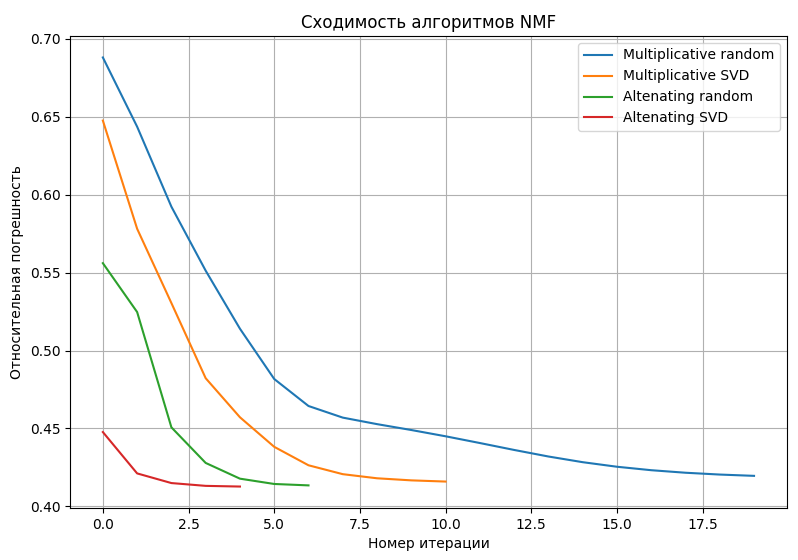
\includegraphics[width=\linewidth]{assets/Graph1.png}
  \caption{График относительной погрешности}
  \label{fig:relativeApproximationError}
\end{figure}

На Рис.~\ref{fig:relativeApproximationError} отчётливо видно, что мультипликативным алогритмам необходимо в 2-3 раза больше итераций, чтобы добиться заданной точности. Также график показывает, что мультипликативные алгоритмы чаще сходятся к более ``плохой'' точке локального минимума, которая даёт меньшую точность разложения. Касательно алгоритмов попеременных наименьших квадратов видно, что даже после первой итерации относительная ошибка значительно меньше чем у предыдущих алгоритмов и в целом они требуют намного меньше итераций.

В обоих случаях инициализация матриц $W$ и $H$ с помощью сингулярного разложения понижает ошибку на первой итерации и уменьшает количество итерации.


\newpage


Ниже приведены данные показывающие затраты по времени на выполнение алгоритмов:

\verbatimfont{\small}
\begin{verbatim}
# Initialization:
Random takes 2.002e-05s
SVD takes 4.435e-04s
# Methods:
Multiplicative random takes 3.202e-03s
Multiplicative SVD takes 6.939e-04s
Altenating random takes 1.151e-02s
Altenating SVD takes 6.742e-03s
\end{verbatim}

Ниже приведени результаты алгоритма попеременных наименьших квадратов с использованием SVD инициализации:

\begin{align*}
W H = 
\begin{pmatrix}
     0.153  &   0  &   0.089 \\
     0  &   0  &   0.518 \\
     0  &   0  &   0.518 \\ 
     0.372  &   0.099  &   0 \\
     0.237  &   0  &   0 \\
     0  &   0.516  &   0 \\ 
     0.525  &  	0  &   0.027 \\
     0.042  &   0.752  &   0 \\
     0.229  &   0.131  &   0.613 \\
     0.042  &   0.752  &   0
\end{pmatrix}
\begin{pmatrix}
     2.152  &   0  &   1.897  &   1.530  &  0 \\
     0  &   1.472  &   1.022  &   0  &   0 \\
     0  &   0  &   0.250  &   0.493  &   1.844
\end{pmatrix}
\end{align*}

 Представим полученные данные в виде таблиц:

\begin{center}
 \begin{tabular}{ l | c c c c c c } 
 Термин      & 1 & 2 & 3 \\
 \hline
 eigenvalue  & 0.153  &   0  &   0.089 \\
 England     & 0  &   0  &   0.518 \\
 FIFA        & 0  &   0  &   0.518 \\ 
 Google      & 0.372  &   0.099  &   0 \\
 Internet    & 0.237  &   0  &   0 \\
 link        & 0  &   0.516  &   0 \\ 
 matrix      & 0.525  &  	0  &   0.027 \\
 page        & 0.042  &   0.752  &   0 \\
 rank        & 0.229  &   0.131  &   0.613 \\
 Web         & 0.042  &   0.752  &   0
\end{tabular}
\end{center}

\begin{center}
 \begin{tabular}{ l | c c c c c c } 
 Вектор      & Док 1 & Док 2 & Док 3 & Док 4 & Док 5 \\
 \hline
 1           & 2.152  &   0  &   1.897  &   1.530  &  0 \\ 
 2           & 0  &   1.472  &   1.022  &   0  &   0 \\
 3           & 0  &   0  &   0.250  &   0.493  &   1.844 \\ 
\end{tabular}
\end{center}


Напомним, что первые четыре документа рассказывают о Google и рейтинге веб-страниц, а пятый касается футбола. Из таблиц можно увидеть, что первые четыре документа представлены векторами, которые имеют большие компоненты для ключевых слов, связанных с Google. В отличие от этого, пятый документ представлен только третьим базисным вектором, так же с большой компонентой. Мы видим, что третий вектор представляет документы рассказывающие о футболе, а два других показывают документы, связанные с Google.


\newpage


\section{Выводы}

Мультипликативные алгоритмы требуют намного больше итераций, чем альтернативы, такие как алгоритмы попеременных наименьших квадратов, и работа на онду итерацию предельно высока. Каждая итерация требует шесть $O(n^3)$ матрично-матричных умножений полностью плотных матриц и шесть
$O (n^2)$ покомпонентных операций.

Один недостаток мультипликативных алгоритмов состоит в том, что как только элемент в $W$ или $H$ становится 0, он будет оставаться равным 0. Эта блокировка нулевых элементов означает, что, как только алгоритм начинает двигаться по пути к фиксированной точке, даже если это плохая фиксированная точка, он будет продолжать двигаться в том же направлении. 

Алгоритмы ALS являются более гибкими, позволяя итеративному процессу уйти с неправильного пути. В зависимости от реализации алгоритмы ALS могут быть очень быстрыми.


\newpage


\begin{thebibliography}{9}
	\bibitem{berry} Michael W. Berry, Murray Browne, Amy N. Langville, V. Paul Pauca, Robert
J. Plemmons, Algorithms and applications for approximate nonnegative matrix factorization, Computational Statistics; Data Analysis, Volume 52, Issue 1, 2007,
p. 155-173.
	\bibitem{elden} Lars Eldén. 2007. Matrix Methods in Data Mining and Pattern Recognition
(Fundamentals of Algorithms). Soc. for Industrial and Applied Math.,
Philadelphia, PA, USA.
	\bibitem{demmel} Деммель Дж. Вычислительная линейная алгебра. М.: Мир, 2001.
	\bibitem{habr} Интернет ресурс 'Habr'. https://habr.com/ru/post/264375/
\end{thebibliography}

\end{document}